
\chapter{سخت افزار الکترونیکی ربات}

\section{مقدمه}

\section{پردازنده \lr{ARM} سری \lr{f101c8t6}}

شاید واژه
\lr{ARM}
\noindent\unskip\LTRfootnote{Advanced RISC Machine}
برایتان آشنا باشد.
\lr{ARM}
نوعی معماری برای ساخت انواع پردازنده‌های 32 و 64 بیتی است. از دلایل محبوبیت و استفاده از پردازنده‌هایی با این معماری در انواع سیستم‌های نهفته
\noindent\unskip\LTRfootnote{Embedded Systems}،
می‌توان به قیمت مناسب، سرعت بالاتر، توان مصرفی پایین و... اشاره کرد. عدد بعد از این حروف نشانگر تعداد خطوط اجرایی
\noindent\unskip\LTRfootnote{performance lines}
پردازنده می‌باشد. یکی از شرکت‌هایی که این معماری را برای ساخت پردازنده های خود انتخاب می‌کند، شرکت
\lr{ST}
می‌باشد. میکروکنترلرهای این شرکت تحت عنوان
\lr{STM}
بعلت تنوع بالا و ارائه کتابخانه های برنامه‌نویسی کاربردی، بسیار مشهور شده‌اند.

\begin{figure}[H]
	\centering
	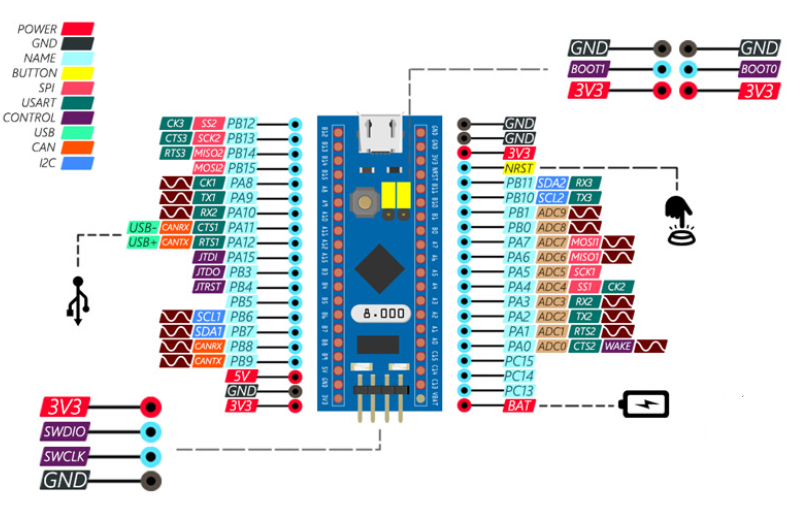
\includegraphics[width=1\textwidth]{./images/Chapter4/STM32Pinout}
	\caption[]{ \cite{STM32F101}}
	\label{پایه‌های آرم}
\end{figure}


\section{ماژول \lr{ESP32-CAM}}

ماژول
\lr{ESP32-CAM}
یک ماژول کامل است که برای بسیاری از کاربردهای صنعتی و اینترنت اشیاء استفاده می‌شود. همچنین دارای قابلیت‌های متعددی اعم از انواع ارتباطات، ذخیره‌سازی اطلاعات و... بوده و دارای مشخصات فنی زیر می‌باشد:
% \cite{ESP32details}
\begin{itemize}
	\item 
	ارتباطات: بلوتوث 4.2 \lr{BLE} به همراه \lr{Wifi 802.11b}. که از بارگذاری تصویر از طریق \lr{WiFi} پشتیبانی می کند.
	\item
	اتصالات: \lr{UART} ، \lr{SPI} ، \lr{I2C}، و \lr{PWM} و دارای 9 پایه \lr{GPIO} است.
	\item
	فرکانس ساعت: تا 160 مگاهرتز
	\item
	قدرت محاسباتی میکروکنترلر: حداکثر 600 \lr{DMIPS}.
	\item
	حافظه: 520 کیلوبایت \lr{SRAM}، چهار مگابایت حافظه کارت \lr{PSRAM + SD}
	\item
	دوربین: از دوربین های \lr{OV2640} پشتیبانی می‌کند که دارای 2 مگاپیکسل روی سنسور با اندازه آرایه  1622 × 1200\lr{UXGA} پیکسل هستند.
\end{itemize}



برای اتصال این ماژول به کامپیوتر و برنامه‌ریزی
\noindent\unskip\LTRfootnote{Programming}
آن می‌توان از دو روش استفاده کرد:

1-استفاده از یک مبدل \lr{USB} به سریال مانند

2-استفاده از یک برد دیگر مانند آردوینو
\noindent\unskip
\noindent\unskip\RTLfootnote{برای برنامه‌ریزی از طریق ارتباطاتی همچون \lr{UART}}


\begin{figure}[H]
	\centering
	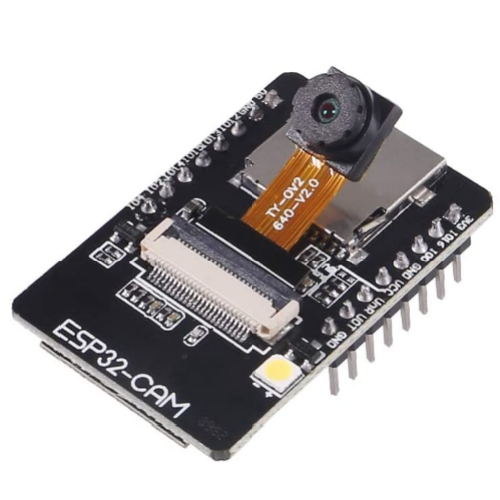
\includegraphics[width=0.4\textwidth]{./images/Chapter4/ESP32CAM}
	\caption[ماژول \lr{ESP32CAM}]{ماژول \lr{ESP32CAM} \cite{ESP32CAM}}
	\label{ماژول ای اس پی}
\end{figure}

نکته بسیار مهم اینکه برای برنامه ریزی شدن این ماژول باید حتما حین برنامه ریزی دو پایه ی \lr{Io0} و\lr{GND} به یکدیگر متصل باشند. همچنین پس از تکمیل برنامه ریزی باید اتصال این دو پایه را قطع کرد.\\ 

\section{دوربین \lr{OV2640}}
دوربین \lr{OV2640} یک سنسور تصویر \lr{CMOS} با رزولوشن بالا است که توسط شرکت \lr{OmniVision} تولید می‌شود.این دوربین به ویژه برای برنامه‌هایی مناسب است که نیاز به تصاویر با کیفیت بالا و ویژگی‌های پیشرفته دارند. از آنجا که این دوربین بسیار محبوب و پرطرفدار است، در بسیاری از پروژه‌های الکترونیک و رباتیک استفاده می‌شود، از جمله پروژه‌هایی که به آن اشاره کردید، یعنی ربات عنکبوتی چهار پا.


\begin{figure}[h]
	\centering
	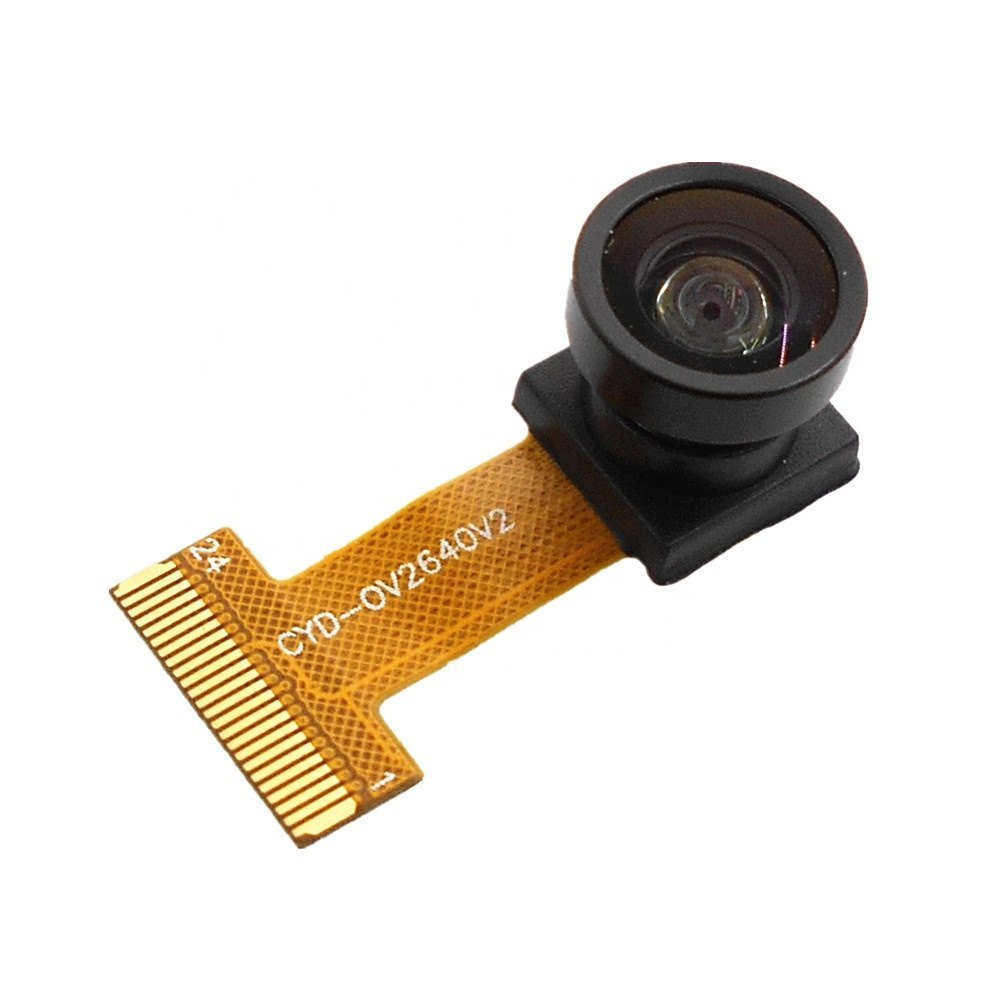
\includegraphics[width=0.4\textwidth]{./images/Chapter4/OV2640}
	\caption[دوربین \lr{OV2640}]{دوربین \lr{OV2640} \cite{OV2640}}
	\label{عکس دوربین}
\end{figure}

ویژگی‌های کلیدی دوربین \lr{OV2640} عبارت‌اند از:
\begin{itemize}
	\item
	رزولوشن بالا: دوربین \lr{OV2640} قابلیت ثبت تصاویر با رزولوشن بالا را دارد. این دوربین قابلیت ثبت تصاویر با رزولوشن حداکثر 2 مگاپیکسل ($1200 \times 1600$) را دارد.
	
	\item
	فرمت تصویری متنوع: این دوربین از فرمت‌های مختلف تصویری مانند \lr{RGB} ، \lr{YUV} ، \lr{JPEG} و \lr{Raw}  پشتیبانی می‌کند که این امر به کاربر امکان انتخاب فرمتی مناسب با توجه به نیازهای پروژه را می‌دهد.
	\item
	تمرکز اتوماتیک \lr{(Auto-Focus)}: دوربین \lr{OV2640} دارای ویژگی تمرکز اتوماتیک بر روی تصاویر است که بهترین تنظیمات فوکوس را برای صحنه‌ها و شرایط مختلف فراهم می‌کند.
	\item
	تنظیمات تصویری: این دوربین اجازه تنظیمات مختلف تصویری مانند شدت روشنایی \lr{(Exposure)}, توازن رنگ \lr{(White Balance)}, کنتراست \lr{(Contrast)} و... را به کاربر می‌دهد.
	\item
	حالت تصویربرداری پیوسته \lr{(Continuous Shooting)}: با امکان ثبت تصاویر به صورت پیوسته، دوربین \lr{OV2640} مناسب برای برنامه‌هایی است که نیاز به ثبت تصاویر متوالی دارند.
	\item
	حالت‌های مختلف عکسبرداری: این دوربین از حالت‌های مختلف عکسبرداری مانند \lr{Single Capture}، \lr{Raw Capture} و \lr{JPEG Capture} پشتیبانی می‌کند.
	\item
	پشتیبانی از ارتباطات: دوربین \lr{OV2640} از ارتباطات مختلف مانند \lr{I2C} ، \lr{UART} و \lr{SPI} پشتیبانی می‌کند که این امر ارتباط آسان با میکروکنترلرها و ماژول‌های دیگر را ممکن می‌سازد.
	\item
	کاربرد وسیع: دوربین \lr{OV2640} به عنوان یک ماژول کوچک و قابل حمل، در بسیاری از پروژه‌های رباتیک، دوربین‌های مدار بسته، دوربین‌های امنیتی، دستگاه‌های پزشکی و سایر برنامه‌های صنعتی و مصرفی مورد استفاده قرار می‌گیرد.
\end{itemize}
با توجه به ویژگی‌های برتر دوربین \lr{OV2640}، می‌توان آن را به عنوان یک گزینه مناسب برای پروژه‌های شما در زمینه‌های رباتیک و دید کامپیوتری در نظر گرفت.

\section{سروموتور}
سروموتورها از جمله اجزاء اساسی در رباتیک و به‌ویژه در ربات‌های چهارپا مورد استفاده قرار می‌گیرند. این اجزا جهت کنترل و حرکت اندام‌ها و پاهای ربات به کار می‌روند. سروموتورها معمولاً دارای یک شفت قابل چرخش هستند که از طریق یک سیگنال کنترلی به جلو و عقب حرکت می‌کنند. سروموتورها به دلیل دقت، سرعت و کاربرد‌های متعددشان، بخش مهمی از طراحی و ساخت ربات‌های چهارپا را تشکیل می‌دهند.

در ربات‌های چهارپا، سروموتورها به‌عنوان موتورهای اصلی برای حرکت پاها و اندام‌ها عمل می‌کنند. این سروموتورها معمولاً دقیق و قابل کنترل با سرعت متغیر هستند، که این ویژگی‌ها امکان جابه‌جایی دقیق و پیچیده را فراهم می‌کنند. سروموتورها معمولاً با استفاده از میکروکنترلرها به راحتی کنترل می‌شوند. این اجزا به تنهایی یا به صورت گروهی در ربات‌های چهارپا استفاده می‌شوند تا حرکت و موقعیت دقیق در سیستم رباتیک تضمین شود.

\begin{figure}[h]
	\centering
	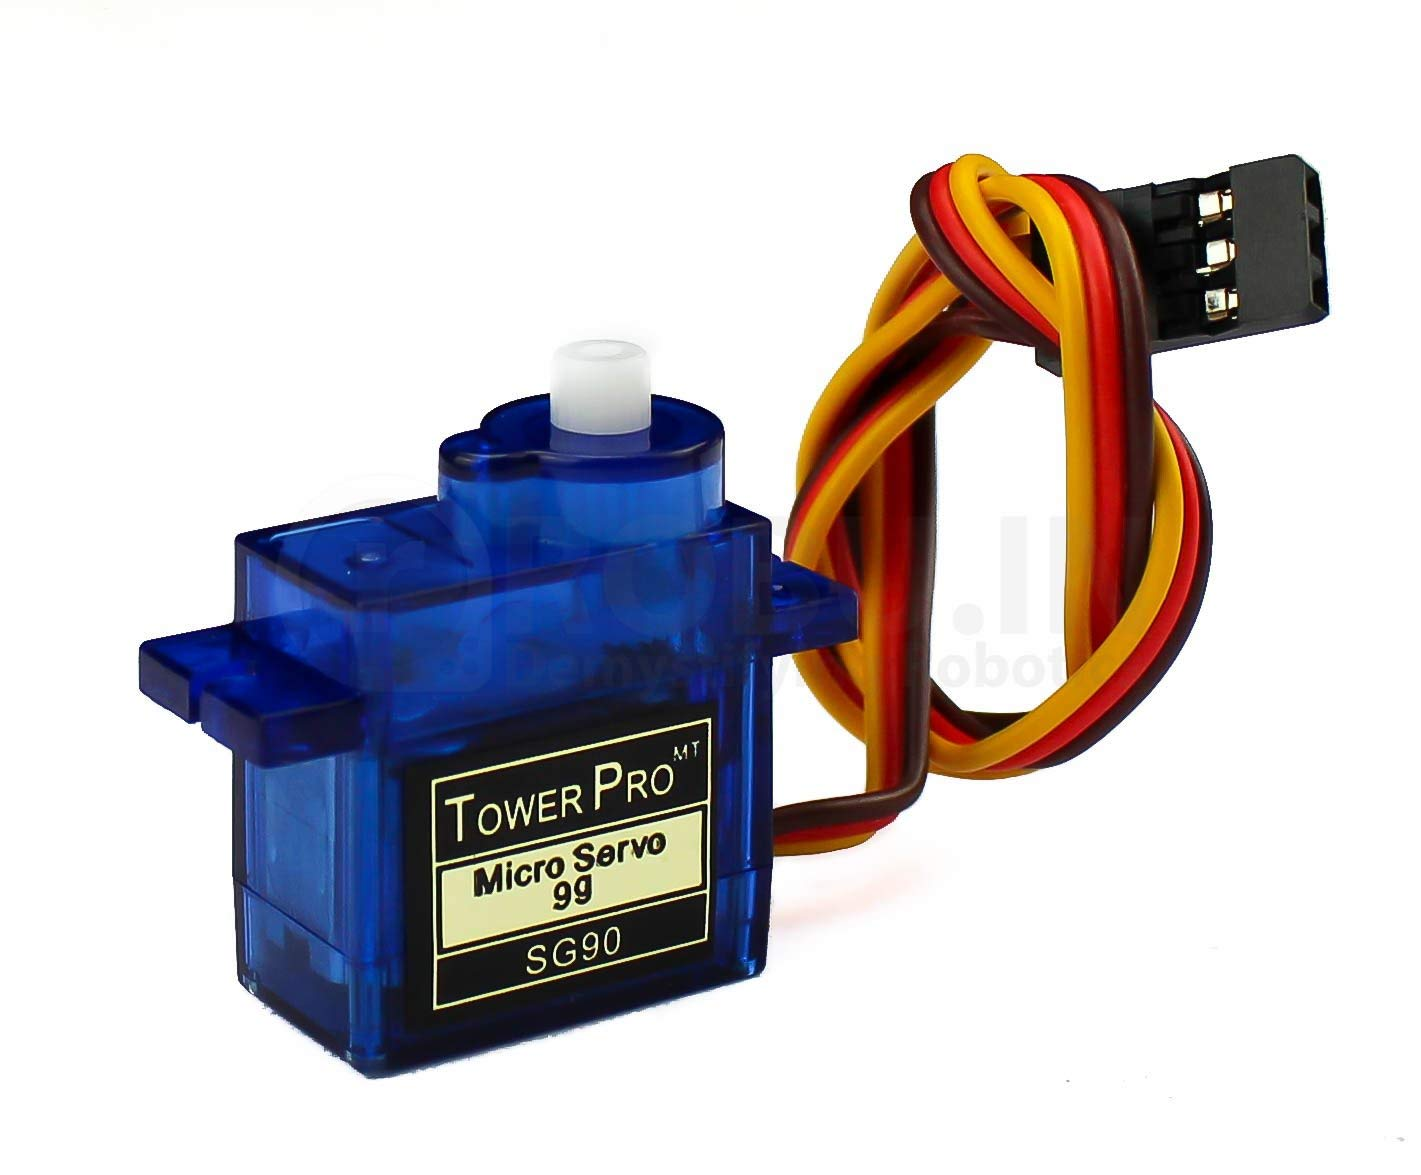
\includegraphics[width=0.4\textwidth]{./images/Chapter4/ServoMotor}
	\caption[سروموتور \lr{SG90}]{سروموتور \lr{SG90} \cite{ServoMotor}}
	\label{سروموتور}
\end{figure}

\subsection{روش \lr{PWM}}
\subsubsection{مدولاسیون چیست؟}
احتمالا عبارت‌های \lr{AM} و \lr{FM} را روی وسایل الکتریکی مانند رادیو و... مشاهده کرده اید.عبارت \lr{AM}، مخفف \lr{Amplitude Modulation} به‌معنی مدولاسیون دامنه و عبارت \lr{FM} مخفف مدولاسیون فاز است. مدولاسیون دامنه، راهی برای ارسال یک سیگنال روی یک حامل است.مدولاسیون اساساً یک راه برای رمزگذاری یک سیگنال بر روی سیگنال حامل است.

به عبارت دیگر مدولاسیون سوار کردن سیگنال مورد نظر بر روی یک سیگنال دیگر است. اینکار به‌منظور افزایش برد سیگنال و بهره‌وری انتقال انجام می‌شود. به‌طور کلی، فرایند گنجاندن سیگنال حاوی اطلاعات در سیگنالی دیگر را مدولاسیون می‌نامند.

\subsubsection{مدولاسیون پهنای پالس}
مدولاسیون پهنای پالس یا \lr{PWM} ، نوعی سیگنال است که می‌توان آن را توسط یک مدار مجتمع دیجیتال مانند میکروکنترلر تولید کرد. این سیگنال تولیدی یک قطار پالس بوده و یک شکل‌موج مربعی را تشکیل می‌دهند. به عبارتی در هر زمان مشخص، سیگنال تنها می‌تواند دو وضعیت بالا \lr{(High)} که معادل 1 دیجیتالی و یا پایین \lr{(Low)} که معادل صفر دیجیتالی است را به خود اختصاص دهد.

مدت‌زمانی که سیگنال در وضعیت \lr{High} قرار دارد، «زمان روشن» \lr{(On Time)}و مدت‌زمانی که سیگنال در وضعیت \lr{Low} است، «زمان خاموش» \lr{(Off Time)} نامیده می‌شود.

\section{تجهیزات مکانیکی}

\subsection{سایر قطعات متصل کننده}
پین هدر ها و ...

\section{جمع بندی}
همانطور که در بخش های این فصل بررسی شد، تمامی سخت‌افزار های استفاده شده در پروژه اعم از الکترونیکی و یا مکانیکی و یا سایر تجهیزات همگی با در نظر گرفتن کاربری تا حدامکان بصورت اقتصادی انتخاب شده و همچنین قابل دسترس در بازار ایران می‌باشند.
از سوی دیگر داشتن شناخت کافی از جزئیات و اطلاعات فنی هریک از سخت‌افزار‌ها منجر به انتخاب  قطعات معرفی شده در کمترین زمان ممکن انجامید.

